\documentclass[12pt,a4paper]{article}

% ============================================================
% PACKAGES
% ============================================================
\usepackage[vietnamese]{babel}
\usepackage{geometry}
\usepackage{amsmath, amssymb, amsthm}
\usepackage{graphicx}
\usepackage{booktabs}
\usepackage{array}
\usepackage{longtable}
\usepackage{xcolor}
\usepackage{listings}
\usepackage{hyperref}
\usepackage{enumitem}
\usepackage{fancyhdr}
\usepackage{titlesec}
\usepackage[most]{tcolorbox}
\usepackage{listings}
\usepackage{float}
\usepackage{multirow}
\usepackage{caption}
\usepackage{subcaption}
\usepackage{tabularx}
\usepackage[authoryear]{natbib}
\usepackage{setspace}
\usepackage{mathtools}
\usepackage{fontspec}
\usepackage{bookmark}
\usepackage{xurl}

% XeLaTeX font setup. Tries Times New Roman first, then safe Overleaf fonts.
\IfFontExistsTF{Times New Roman}{%
  \setmainfont{Times New Roman}%
}{%
  \IfFontExistsTF{Tinos}{%
    \setmainfont{Tinos}%
  }{%
    \IfFontExistsTF{FreeSerif}{\setmainfont{FreeSerif}}{\setmainfont{Liberation Serif}}%
  }%
}

\captionsetup{font=small, labelfont=bf}

% ============================================================
% PAGE LAYOUT
% ============================================================
\geometry{
  top=2.5cm, bottom=2.5cm,
  left=3cm, right=2.5cm
}
\setstretch{1.3}
\setlength{\parindent}{0pt}
\setlength{\parskip}{6pt plus 2pt minus 1pt}
\setcounter{tocdepth}{3}
\setcounter{secnumdepth}{0}

% ============================================================
% COLORS
% ============================================================
\definecolor{mainblue}{RGB}{0, 70, 127}
\definecolor{lightblue}{RGB}{220, 235, 250}
\definecolor{darkgray}{RGB}{50, 50, 50}
\definecolor{codegreen}{RGB}{0, 120, 0}
\definecolor{codered}{RGB}{180, 0, 0}
\definecolor{codegray}{rgb}{0.5,0.5,0.5}
\definecolor{codeback}{rgb}{0.97,0.97,0.97}
\definecolor{formulabg}{RGB}{245, 248, 255}
\definecolor{codebg}{RGB}{248,248,248}
\definecolor{codeframe}{RGB}{220,220,220}
\definecolor{codecomment}{RGB}{100,100,100}
\definecolor{codestring}{RGB}{163,21,21}
\definecolor{codekeyword}{RGB}{0,0,200}
\definecolor{outputbg}{RGB}{240,248,255}

\lstdefinestyle{Rstyle}{
  language        = R,
  backgroundcolor = \color{codebg},
  frame           = single,
  framesep        = 4pt,
  rulecolor       = \color{codeframe},
  basicstyle      = \ttfamily\small,
  keywordstyle    = \color{codekeyword}\bfseries,
  stringstyle     = \color{codestring},
  commentstyle    = \color{codecomment}\itshape,
  showstringspaces= false,
  breaklines      = true,
  breakatwhitespace=true,
  tabsize         = 2,
  numbers         = left,
  numberstyle     = \tiny\color{gray},
  numbersep       = 6pt,
  xleftmargin     = 15pt,
}

\lstdefinestyle{output}{
  backgroundcolor = \color{outputbg},
  frame           = single,
  framesep        = 4pt,
  rulecolor       = \color{codeframe},
  basicstyle      = \ttfamily\small,
  breaklines      = true,
  numbers         = none,
  xleftmargin     = 8pt,
}

% ============================================================
% UNICODE HELPERS FOR TEXT COPIED FROM WORD
% ============================================================

\renewcommand{\contentsname}{Mục lục}
\hypersetup{
  pdftitle={Tự tương quan trong mô hình hồi quy tuyến tính bội},
  hidelinks,
  pdfcreator={LaTeX}}

% ============================================================
% MATH HELPERS
% ============================================================
\DeclareMathOperator{\E}{E}
\DeclareMathOperator{\Var}{Var}
\DeclareMathOperator{\Cov}{Cov}
\DeclareMathOperator{\SE}{SE}


% Graphics scaling from pandoc export
\makeatletter
\def\maxwidth{\ifdim\Gin@nat@width>\linewidth\linewidth\else\Gin@nat@width\fi}
\def\maxheight{\ifdim\Gin@nat@height>\textheight\textheight\else\Gin@nat@height\fi}
\makeatother
\setkeys{Gin}{width=\maxwidth,height=\maxheight,keepaspectratio}
\providecommand{\tightlist}{\setlength{\itemsep}{0pt}\setlength{\parskip}{0pt}}

\title{\textbf{Tự tương quan trong mô hình hồi quy tuyến tính bội}}
\author{}
\date{Ngày 23 tháng 5 năm 2026}

\begin{document}
\maketitle

{
\setcounter{tocdepth}{3}
\tableofcontents
}
\section{1. Khái niệm và cơ sở lý thuyết của tự tương
quan}\label{khuxe1i-niux1ec7m-vuxe0-cux1a1-sux1edf-luxfd-thuyux1ebft-cux1ee7a-tux1ef1-tux1b0ux1a1ng-quan}

\subsection{1.1. Mô hình hồi quy tuyến tính bội và sai số ngẫu
nhiên}\label{nhux1eafc-lux1ea1i-muxf4-huxecnh-hux1ed3i-quy-tuyux1ebfn-tuxednh-bux1ed9i-vuxe0-sai-sux1ed1-ngux1eabu-nhiuxean}

Xét \(y_i , . . . , y_n\) là n giá trị quan trắc độc lập của Y . Khi đó, mỗi \(y_i\) có
thể biểu diễn dưới dạng

\[
y_i = \beta_0 + \beta_1x_{1i} + \beta_2x_{2i} + \cdots + \beta_jx_{ji} + \varepsilon_i,\quad i = 1,2,\ldots,n
\]

Trong đó:

\begin{itemize}
\item
  \(y_i\) là giá trị của biến phụ thuộc tại quan trắc thứ i.
\item
  \(x_{1i}\), \(x_{2i}\), ..., \(x_{ji}\) là giá trị của các biến độc lập thứ j tại quan trắc thứ
  i.
\item
  \(\beta_0\) là hệ số chặn của mô hình.
\item
  \(\beta_1\), \(\beta_2\), ..., \(\beta_j\) là các hệ số hồi quy cần ước lượng.
\item
  \(\varepsilon_i\) là sai số ngẫu nhiên tại quan trắc thứ i, tức phần biến động của \(y_i\)
  mà mô hình chưa giải thích được.
\item
  j là số biến độc lập; n là số quan trắc.
\end{itemize}

\subsection{1.2. Giả định không tự tương
quan}\label{giux1ea3-ux111ux1ecbnh-khuxf4ng-tux1ef1-tux1b0ux1a1ng-quan}

Trong mô hình hồi quy tuyến tính cổ điển, sai số thường được giả định có
kỳ vọng bằng 0, phương sai không đổi và không có tương quan giữa các
quan trắc khác nhau:

\[
\operatorname{E}(\varepsilon_i)=0
\]
\[
\operatorname{Var}(\varepsilon_i)=\sigma^2
\]
\[
\operatorname{Cov}(\varepsilon_i,\varepsilon_j)=0,\quad i\neq j
\]

Trong đó:

\begin{itemize}
\item
  \(\operatorname{E}(\varepsilon_i)\) là kỳ vọng của sai số tại quan trắc thứ i.
\item
  \(\operatorname{Var}(\varepsilon_i)\) là phương sai của sai số tại quan trắc thứ i.
\item
  \(\sigma^2\) là phương sai chung của sai số.
\item
  \(\operatorname{Cov}(\varepsilon_i,\varepsilon_j)\) là hiệp phương sai giữa sai số tại hai quan trắc i và j.
\item
  \(i\neq j\) nghĩa là hai quan trắc khác nhau.
\end{itemize}

Điều kiện \(\operatorname{Cov}(\varepsilon_i,\varepsilon_j)\) = 0 cho biết sai số ở một quan trắc không có quan
hệ tuyến tính với sai số ở quan trắc khác. Đây chính là giả định không
tự tương quan hoặc giả định độc lập theo nghĩa không tương quan của sai
số.

\subsection{1.3. Khái niệm tự tương quan}

Tự tương quan là hiện tượng sai số của quan sát thứ $i$ có quan hệ với sai số của quan sát thứ $j$, với $i \neq j$. Khi đó, giả định các sai số độc lập với nhau bị vi phạm.

Về mặt toán học, hiện tượng tự tương quan được biểu diễn bởi:

\[
\operatorname{Cov}(\varepsilon_i,\varepsilon_j) \neq 0,
\qquad i \neq j
\]

Trong đó, $\operatorname{Cov}(\varepsilon_i,\varepsilon_j)$ biểu thị hiệp phương sai giữa sai số của quan sát thứ $i$ và sai số của quan sát thứ $j$.

Tùy theo cách các quan sát có thứ tự hoặc có mối liên hệ với nhau, tự tương quan có thể xuất hiện dưới hai dạng chính:

\begin{itemize}
    \item \textbf{Tự tương quan theo thời gian}: sai số tại một thời điểm có quan hệ với sai số tại những thời điểm khác.
    
    \item \textbf{Tự tương quan theo không gian}: sai số của các quan sát ở gần nhau hoặc thuộc cùng một khu vực có quan hệ với nhau.
\end{itemize}

\textbf{Ví dụ: Hồi quy giá thuê nhà tại TP.HCM}

Giả sử ta xây dựng mô hình hồi quy để giải thích giá thuê của các căn nhà tại Quận 1 và Hóc Môn dựa trên diện tích nhà và số phòng ngủ:

Mô hình dựa trên diện tích nhà và số phòng ngủ:

\[
\mathrm{Rent}_i
=
\beta_0
+
\beta_1 \mathrm{Area}_i
+
\beta_2 \mathrm{Bedroom}_i
+
\varepsilon_i
\]

Trong đó, $\mathrm{Rent}_i$ là giá thuê của căn nhà thứ $i$,
$\mathrm{Area}_i$ là diện tích nhà,
$\mathrm{Bedroom}_i$ là số phòng ngủ
và $\varepsilon_i$ là sai số của mô hình.

Nếu không có tự tương quan, sai số của một căn nhà không có quan hệ với sai số của căn nhà khác. việc mô hình dự đoán giá thuê của một căn nhà tại Quận 1 cao hơn hoặc thấp hơn thực tế không cho biết trước mô hình sẽ dự đoán như thế nào đối với căn nhà khác. Đối với căn nhà khác, mô hình có thể dự đoán cao hơn thực tế, thấp hơn thực tế hoặc cũng có thể dự đoán gần chính xác.

Tuy nhiên, giá thuê nhà còn chịu ảnh hưởng bởi khu vực. Nếu mô hình không đưa biến khu vực vào, những ảnh hưởng đặc trưng của từng khu vực sẽ được phản ánh một phần trong sai số $\varepsilon_i$. Do các căn nhà trong cùng khu vực cùng chịu tác động từ các yếu tố như vị trí, mức độ thuận tiện, cơ sở hạ tầng và nhu cầu thuê, sai số của chúng có thể có xu hướng tương tự nhau. Khi đó, giả định các sai số độc lập bị vi phạm.

\textbf{Ví dụ: Hồi quy doanh thu bán hàng}

Giả sử ta xây dựng mô hình hồi quy để giải thích doanh thu bán hàng theo tháng dựa trên chi phí quảng cáo và mức giảm giá:

\[
\mathrm{Sales}_t
=
\beta_0
+
\beta_1 \mathrm{Advertising}_t
+
\beta_2 \mathrm{Discount}_t
+
\varepsilon_t
\]

Trong đó, $\mathrm{Sales}_t$ là doanh thu tại tháng $t$, $\mathrm{Advertising}_t$ là chi phí quảng cáo, $\mathrm{Discount}_t$ là mức giảm giá và $\varepsilon_t$ là sai số của mô hình.

Nếu không có tự tương quan, sai số tại một tháng không có quan hệ có hệ thống với sai số tại tháng khác. Việc mô hình dự đoán doanh thu của tháng này cao hơn hoặc thấp hơn thực tế không cho biết trước mô hình sẽ dự đoán như thế nào đối với tháng tiếp theo.

Tuy nhiên, vào những tháng cuối năm, nhu cầu mua sắm thường tăng do người tiêu dùng chuẩn bị cho các dịp lễ và năm mới. Nếu mô hình không đưa yếu tố mùa vụ cuối năm vào, ảnh hưởng này sẽ được phản ánh trong sai số $\varepsilon_t$. Doanh thu thực tế trong nhiều tháng cuối năm liên tiếp có thể cao hơn mức mô hình dự đoán, làm sai số của các tháng này có xu hướng tương tự nhau. Khi đó, giả định các sai số độc lập theo thời gian bị vi phạm.


\subsection{1.4. Sai số và thặng dư sau ước lượng}

Trong mô hình hồi quy, hiện tượng tự tương quan được định nghĩa trên các sai số ngẫu nhiên $\varepsilon_i$. Tuy nhiên, trong thực tế, ta không thể quan sát trực tiếp $\varepsilon_i$ vì các tham số tổng thể $\beta_0,\beta_1,\ldots,\beta_j$ chưa biết.

Sau khi ước lượng mô hình từ dữ liệu mẫu, ta thu được các hệ số ước lượng
$\hat{\beta}_0,\hat{\beta}_1,\ldots,\hat{\beta}_j$ và giá trị dự đoán của quan sát thứ $i$:

\[
\hat{y}_i
=
\hat{\beta}_0
+
\hat{\beta}_1 x_{1i}
+
\hat{\beta}_2 x_{2i}
+
\cdots
+
\hat{\beta}_j x_{ji}
\]

Thặng dư của quan sát thứ $i$ được tính bằng:

\[
e_i
=
y_i-\hat{y}_i
\]

Trong đó:

\begin{itemize}
    \item $e_i$ là thặng dư của quan sát thứ $i$.
    
    \item $y_i$ là giá trị thực tế quan sát được của biến phụ thuộc tại quan sát thứ $i$.
    
    \item $\hat{y}_i$ là giá trị dự đoán từ mô hình hồi quy đã ước lượng tại quan sát thứ $i$.
    
    \item $\hat{\beta}_0,\hat{\beta}_1,\ldots,\hat{\beta}_j$ là các hệ số hồi quy được ước lượng từ dữ liệu mẫu.
\end{itemize}

Dưới dạng vector, thặng dư của toàn bộ mô hình được viết là:

\[
e
=
y-\hat{y}
\]

Thặng dư $e$ được sử dụng như một đại diện gần đúng cho sai số ngẫu nhiên $\varepsilon$. Vì vậy, trong thực hành, việc kiểm tra tự tương quan thường được thực hiện dựa trên các thặng dư thu được từ mô hình hồi quy đã ước lượng.

\section{2. Nguyên nhân dẫn đến tự tương quan}

Dựa trên các nguyên nhân được trình bày bởi Gujarati và Porter (2009), có thể khái quát nguyên nhân dẫn đến tự tương quan thành hai nhóm chính:

\begin{itemize}
    \item Do cấu trúc phụ thuộc vốn có của dữ liệu hoặc của quá trình sai số.
    \item Do mô hình chưa được đặc tả phù hợp.
\end{itemize}

Các nguyên nhân này không loại trừ nhau. Trong thực tế, một mô hình có thể xuất hiện tự tương quan do nhiều nguyên nhân cùng lúc.

\subsection{2.1. Nguyên nhân do cấu trúc phụ thuộc của dữ liệu}

Đối với dữ liệu chuỗi thời gian, các quan sát được ghi nhận liên tiếp theo thời gian nên giá trị hiện tại có thể chịu ảnh hưởng từ quá khứ. Đồng thời, một cú sốc ngẫu nhiên xuất hiện tại một thời điểm có thể tiếp tục ảnh hưởng sang các thời điểm sau, làm sai số giữa các kỳ có tương quan với nhau.

Một số dạng phụ thuộc thường gặp gồm:

\begin{itemize}
    \item \textbf{Quán tính}: các biến kinh tế thường thay đổi từ từ, nên trạng thái tại một thời điểm có xu hướng tiếp tục kéo dài sang các thời điểm sau.
    
    \item \textbf{Tác động có độ trễ}: tác động của một sự kiện hoặc cú sốc có thể không kết thúc ngay lập tức mà tiếp tục ảnh hưởng qua nhiều kỳ.
    
    \item \textbf{Mùa vụ và chu kỳ}: các hoạt động kinh tế có thể lặp lại theo tháng, quý hoặc năm, tạo ra sự phụ thuộc giữa các quan sát theo thời gian.
\end{itemize}

Đối với dữ liệu không gian, các quan sát ở gần nhau hoặc thuộc cùng một khu vực có thể chịu ảnh hưởng từ các điều kiện chung. Vì vậy, sai số của các quan sát có liên hệ về không gian cũng có thể tương quan với nhau.

\subsection{2.2. Nguyên nhân do mô hình chưa được đặc tả phù hợp}

Tự tương quan cũng có thể xuất hiện khi mô hình không phản ánh đúng cấu trúc của dữ liệu. Khi một yếu tố có tính hệ thống bị bỏ sót hoặc được mô hình hóa không phù hợp, ảnh hưởng của yếu tố đó sẽ nằm lại trong sai số và tạo ra mẫu hình tương quan.

Một số nguyên nhân thường gặp gồm:

\begin{itemize}
    \item \textbf{Bỏ sót biến quan trọng}: một biến có ảnh hưởng đến biến phụ thuộc nhưng không được đưa vào mô hình.
    
    \item \textbf{Sai dạng hàm}: mối quan hệ thực tế là phi tuyến nhưng mô hình lại được xây dựng dưới dạng tuyến tính không phù hợp.
    
    \item \textbf{Thao tác hoặc biến đổi dữ liệu}: các phương pháp như làm trơn hoặc nội suy có thể tạo ra sự liên hệ nhân tạo giữa các quan sát.
\end{itemize}

Tóm lại, tự tương quan có thể xuất phát từ cấu trúc phụ thuộc vốn có của dữ liệu hoặc của quá trình sai số. Ngoài ra, nó cũng có thể phát sinh khi mô hình chưa phản ánh đầy đủ cấu trúc của dữ liệu, khiến các yếu tố có tính hệ thống bị đưa vào sai số.


\section{3. Hậu quả thống kê của tự tương
quan}\label{hux1eadu-quux1ea3-thux1ed1ng-kuxea-cux1ee7a-tux1ef1-tux1b0ux1a1ng-quan}

Hậu quả chính của tự tương quan không phải là mô hình không thể ước lượng được các hệ số hồi quy. Trong nhiều trường hợp, OLS vẫn cho phép tính các hệ số ước lượng. Tuy nhiên, khi các sai số có tương quan với nhau, các công thức phương sai, sai số chuẩn và suy luận thống kê thông thường của OLS có thể không còn chính xác.

\subsection{3.1. Tự tương quan làm sai cấu trúc phương sai của vector
sai
số}\label{tux1ef1-tux1b0ux1a1ng-quan-luxe0m-sai-cux1ea5u-truxfac-phux1b0ux1a1ng-sai-cux1ee7a-vector-sai-sux1ed1}

Với mô hình hồi quy tuyến tính bội viết dưới dạng ma trận:

\[
\mathbf{y} = X\boldsymbol{\beta} + \boldsymbol{\varepsilon}
\]

Trong đó:

\(\mathbf{y}\) là vector giá trị quan trắc của biến phụ thuộc.

\(X\) là ma trận các biến độc lập, thường gồm cả cột 1 cho hệ số chặn.

\(\boldsymbol{\beta}\) là vector các hệ số hồi quy cần ước lượng.

\(\boldsymbol{\varepsilon}\) là vector sai số ngẫu nhiên của mô hình.

Trong mô hình hồi quy tuyến tính cổ điển, ta thường giả định vector sai
số có phương sai không đổi và các sai số giữa các quan trắc khác nhau
không tương quan với nhau:

\[
\operatorname{Var}(\boldsymbol{\varepsilon}) = \sigma^2 I
\]

Trong đó:

\(\operatorname{Var}(\boldsymbol{\varepsilon})\) là ma trận phương sai - hiệp phương sai của vector sai số \(\boldsymbol{\varepsilon}\).

\(\sigma^2\) là phương sai chung của sai số.

I là ma trận đơn vị.

Công thức này có hai ý nghĩa. Thứ nhất, các sai số có cùng phương sai
\(\sigma^2\). Thứ hai, các phần tử ngoài đường chéo của ma trận bằng 0. Phần tử
ngoài đường chéo bằng 0 nghĩa là sai số giữa các quan trắc khác nhau
không tương quan với nhau.

Khi giả định này đúng, phương sai của vector hệ số OLS được tính bằng:

\[
\operatorname{Var}(\hat{\boldsymbol{\beta}})=\sigma^2(X'X)^{-1}
\]

Công thức này là nền tảng để tính sai số chuẩn của các hệ số hồi quy.

Tuy nhiên, khi có tự tương quan, các sai số trong vector \(\boldsymbol{\varepsilon}\) có quan hệ
với nhau. Khi đó:

\[
\operatorname{Var}(\boldsymbol{\varepsilon})\neq \sigma^2 I
\]

Ta viết tổng quát hơn:

\[
\operatorname{Var}(\boldsymbol{\varepsilon}) = \Omega
\]

Trong đó \(\Omega\) là ma trận phương sai - hiệp phương sai tổng quát của vector
sai số. Khi có tự tương quan, các phần tử ngoài đường chéo của \(\Omega\) khác 0.

Lúc này, công thức phương sai đúng của OLS có dạng tổng quát:

\[
\operatorname{Var}(\hat{\boldsymbol{\beta}})=(X'X)^{-1}X'\Omega X(X'X)^{-1}
\]

Vì vậy, nếu mô hình có tự tương quan nhưng ta vẫn dùng công thức cũ
\[
\operatorname{Var}(\hat{\boldsymbol{\beta}})=\sigma^2(X'X)^{-1}
\], thì sai số chuẩn của các hệ số hồi quy có thể bị
tính sai.

Đây là cơ chế quan trọng nhất: tự tương quan làm sai cấu trúc phương sai
- hiệp phương sai của vector sai số, từ đó làm sai sai số chuẩn của hệ
số hồi quy.

\subsection{3.2. Sai số chuẩn sai làm kiểm định t và p-value không đáng tin cậy}

Kiểm định t cho từng hệ số hồi quy có dạng:

\[
t
=
\frac{\hat{\beta}_j-b_j}
{\operatorname{SE}(\hat{\beta}_j)}
\]

Trong đó:

\begin{itemize}
    \item $\hat{\beta}_j$ là hệ số hồi quy ước lượng của biến $X_j$.
    
    \item $b_j$ là giá trị của hệ số theo giả thuyết kiểm định, thường bằng 0.
    
    \item $\operatorname{SE}(\hat{\beta}_j)$ là sai số chuẩn của hệ số ước lượng $\hat{\beta}_j$.
\end{itemize}

Do sai số chuẩn nằm trực tiếp ở mẫu số của thống kê t, sai số chuẩn bị tính sai sẽ làm giá trị t tính được khác với giá trị t đúng:

\[
\widehat{\operatorname{SE}}(\hat{\beta}_j)
\text{ sai}
\quad \Rightarrow \quad
|t|
\text{ sai}
\]

Vì p-value được xác định từ giá trị của thống kê t, nên:

\[
|t|
\text{ sai}
\quad \Rightarrow \quad
p\text{-value sai}
\]

Khi đó, dẫn đến việc kết luận một biến có ý nghĩa thống kê trong khi bằng chứng thực tế chưa đủ mạnh, hoặc bỏ qua một biến thực sự có ý nghĩa.


\subsection{3.3. Ước lượng phương sai sai số và hệ số $R^2$ cần được diễn giải thận trọng}

Trong mô hình OLS thông thường, phương sai của sai số được ước lượng từ tổng bình phương phần dư:

\[
\hat{\sigma}^2
=
\frac{SSE}{n-p}
=
\frac{\sum_{i=1}^{n}e_i^2}{n-p}
\]

Trong đó:

\begin{itemize}
    \item $\hat{\sigma}^2$ là phương sai sai số được ước lượng.
    
    \item $SSE=\sum_{i=1}^{n}e_i^2$ là tổng bình phương thặng dư.
    
    \item $n$ là số quan trắc.
    
    \item $p$ là số tham số được ước lượng trong mô hình, bao gồm hệ số chặn.
\end{itemize}

Công thức trên được xây dựng dựa trên các giả định của mô hình hồi quy tuyến tính cổ điển, trong đó các sai số giữa những quan trắc khác nhau không tương quan với nhau.

Khi có tự tương quan, công thức OLS thông thường có thể không phản ánh đúng độ biến động thực tế của sai số. Khi đó, ước lượng phương sai sai số có thể bị đánh giá cao hoặc thấp, tùy thuộc vào cấu trúc tự tương quan và đặc điểm của dữ liệu. Vì $\hat{\sigma}^2$ được sử dụng để tính sai số chuẩn của các hệ số hồi quy, sai lệch này tiếp tục ảnh hưởng đến các kết quả suy luận thống kê.

Hệ số xác định được tính bằng:

\[
R^2
=
1-\frac{SSE}{TSS}
\]

Trong đó:

\begin{itemize}
    \item $SSE$ là tổng bình phương phần dư.
    
    \item $TSS$ là tổng bình phương độ lệch của biến phụ thuộc so với giá trị trung bình.
\end{itemize}

Giá trị $R^2$ chỉ phản ánh tỷ lệ biến động của biến phụ thuộc được mô hình giải thích trong mẫu. $R^2$ không cho biết các sai số có độc lập với nhau hay không.

Vì vậy, một mô hình vẫn có thể có $R^2$ cao nhưng đồng thời tồn tại tự tương quan trong phần dư. Do đó, không nên chỉ dựa vào $R^2$ để kết luận rằng mô hình đã được đặc tả phù hợp hoặc các kết quả suy luận thống kê là đáng tin cậy.


\subsection{3.4. Kiểm định F, khoảng tin cậy và khoảng dự báo bị ảnh hưởng}

Kiểm định F thường được sử dụng để kiểm tra ý nghĩa thống kê chung của các biến độc lập trong mô hình:

\[
F
=
\frac{MSR}{MSE}
=
\frac{SSR/k}{SSE/(n-p)}
\]

Trong đó:

\begin{itemize}
    \item $SSR$ là tổng bình phương hồi quy.
    
    \item $SSE$ là tổng bình phương phần dư.
    
    \item $MSR=SSR/k$ là trung bình bình phương hồi quy.
    
    \item $MSE=SSE/(n-p)$ là trung bình bình phương sai số.
    
    \item $n$ là số quan trắc.
    
    \item $k$ là số biến độc lập.
    
    \item $p=k+1$ là số tham số được ước lượng trong mô hình, bao gồm hệ số chặn.
\end{itemize}

Kiểm định F thông thường được xây dựng dựa trên giả định về cấu trúc phương sai--hiệp phương sai của sai số:

\[
\operatorname{Var}(\boldsymbol{\varepsilon})
=
\sigma^2 I
\]

Khi có tự tương quan, giả định này bị vi phạm. Khi đó, $MSE$ có thể không phản ánh đúng phương sai của sai số và thống kê F được tính theo công thức thông thường có thể không còn tuân theo phân phối F như giả định.

Do đó:

\[
\text{Cấu trúc sai số bị xác định sai}
\quad \Rightarrow \quad
F\text{ và p-value của kiểm định F không đáng tin cậy}
\]

Hướng sai lệch của giá trị F không cố định: kiểm định có thể đánh giá quá cao hoặc quá thấp ý nghĩa thống kê chung của các biến độc lập, tùy thuộc vào cấu trúc tự tương quan.

Khoảng tin cậy cho một hệ số hồi quy thường có dạng:

\[
\hat{\beta}_j
\pm
t_{1-\alpha/2}
\operatorname{SE}(\hat{\beta}_j)
\]

Do độ rộng của khoảng tin cậy phụ thuộc trực tiếp vào sai số chuẩn, khi sai số chuẩn bị tính sai thì biên sai số và khoảng tin cậy cũng bị tính sai:

\[
\operatorname{SE}(\hat{\beta}_j)
\text{ sai}
\quad \Rightarrow \quad
\text{khoảng tin cậy sai}
\]

Khoảng tin cậy có thể quá rộng hoặc quá hẹp, làm mức độ chính xác của hệ số ước lượng không được phản ánh đúng.

Tương tự, khoảng dự báo phụ thuộc vào phương sai sai số và cấu trúc phụ thuộc giữa các sai số. Khi tự tương quan bị bỏ qua, mức độ bất định của dự báo có thể bị đánh giá không chính xác, làm khoảng dự báo quá rộng hoặc quá hẹp.


\section{4. Phát hiện tự tương quan}

Do sai số ngẫu nhiên thực tế $\varepsilon_i$ không thể quan sát trực tiếp, việc phát hiện tự tương quan thường được thực hiện dựa trên các thặng dư $e_i$ thu được sau khi ước lượng mô hình.

Việc lựa chọn phương pháp phát hiện phụ thuộc vào mối liên hệ tự nhiên giữa các quan sát. Đối với dữ liệu chuỗi thời gian, các quan sát có thứ tự theo thời gian. Đối với dữ liệu không gian, các quan sát có thể liên hệ với nhau thông qua vị trí địa lý, khoảng cách hoặc việc cùng thuộc một khu vực.

Phương pháp đồ thị được sử dụng để nhận diện các mẫu hình ban đầu trong thặng dư. Kiểm định runs kiểm tra xem thứ tự dấu của các thặng dư có mang tính ngẫu nhiên hay không. Đối với dữ liệu chuỗi thời gian, có thể sử dụng thêm kiểm định Durbin--Watson và Breusch--Godfrey để đưa ra kết luận định lượng.


\subsection{4.1. Phương pháp đồ thị}

Phương pháp đồ thị được sử dụng để kiểm tra xem các thặng dư có phân bố ngẫu nhiên hay tạo thành mẫu hình có hệ thống giữa các quan sát hay không.

Cách biểu diễn đồ thị phụ thuộc vào loại dữ liệu và mối liên hệ giữa các quan sát.


\subsubsection{4.1.1. Vẽ thặng dư theo thời gian}

Đối với dữ liệu chuỗi thời gian, ta vẽ thặng dư $e_t$ theo thời điểm $t$ và quan sát sự phân bố của chúng quanh đường $0$.

Nếu không có tự tương quan, các thặng dư thường phân bố tương đối ngẫu nhiên quanh đường $0$, không tạo thành xu hướng hoặc mẫu hình rõ ràng.

Nếu nhiều thặng dư dương hoặc nhiều thặng dư âm xuất hiện liên tiếp thành từng nhóm theo dạng:
\[
+,\;+,\;+,\;-,\;-,\;-
\]
ta nghi ngờ có tự tương quan dương. Khi đó, thặng dư tại các thời điểm gần nhau có xu hướng cùng dấu.

Nếu các thặng dư thường xuyên đảo dấu theo dạng:
\[
+,\;-,\;+,\;-,\;+,\;-
\]
ta nghi ngờ có tự tương quan âm.

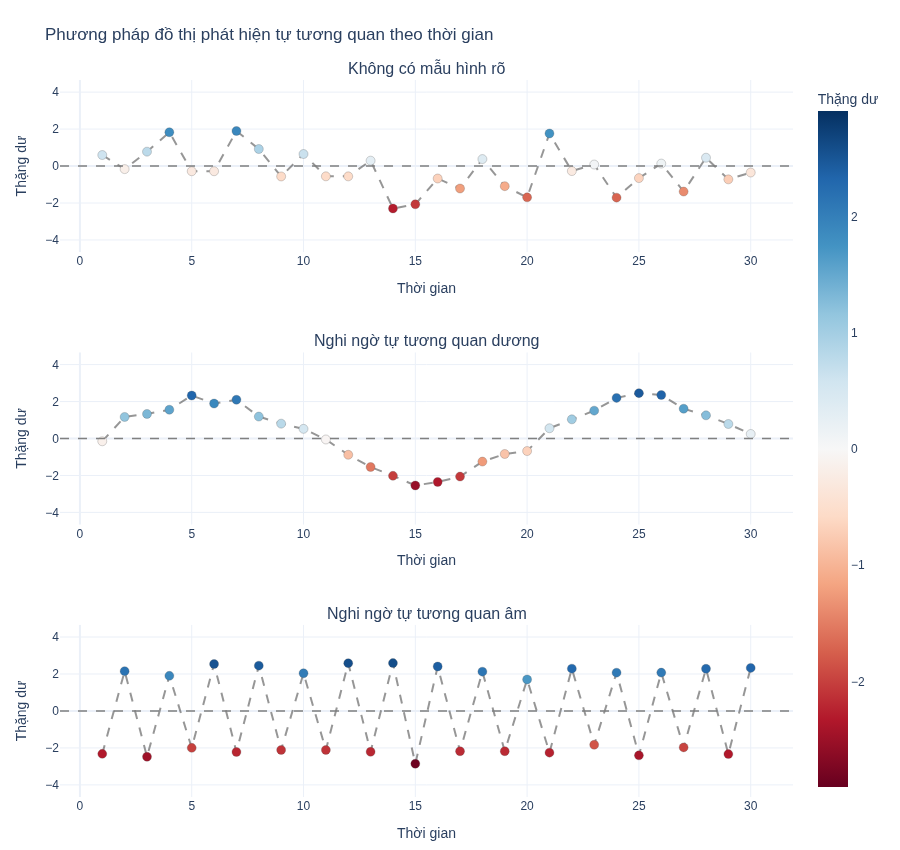
\includegraphics{media/plot_ts.png}

\subsubsection{4.1.2. Vẽ thặng dư theo vị trí hoặc khu vực}

Đối với dữ liệu không gian, có thể biểu diễn thặng dư theo vị trí địa lý hoặc theo từng khu vực.

Nếu các quan sát ở gần nhau hoặc thuộc cùng một khu vực có thặng dư tương tự nhau, chẳng hạn cùng dương hoặc cùng âm, ta nghi ngờ có tự tương quan theo không gian.

Nếu thặng dư phân bố ngẫu nhiên giữa các vị trí và không tạo thành các cụm rõ ràng, ta chưa thấy dấu hiệu tự tương quan theo không gian.

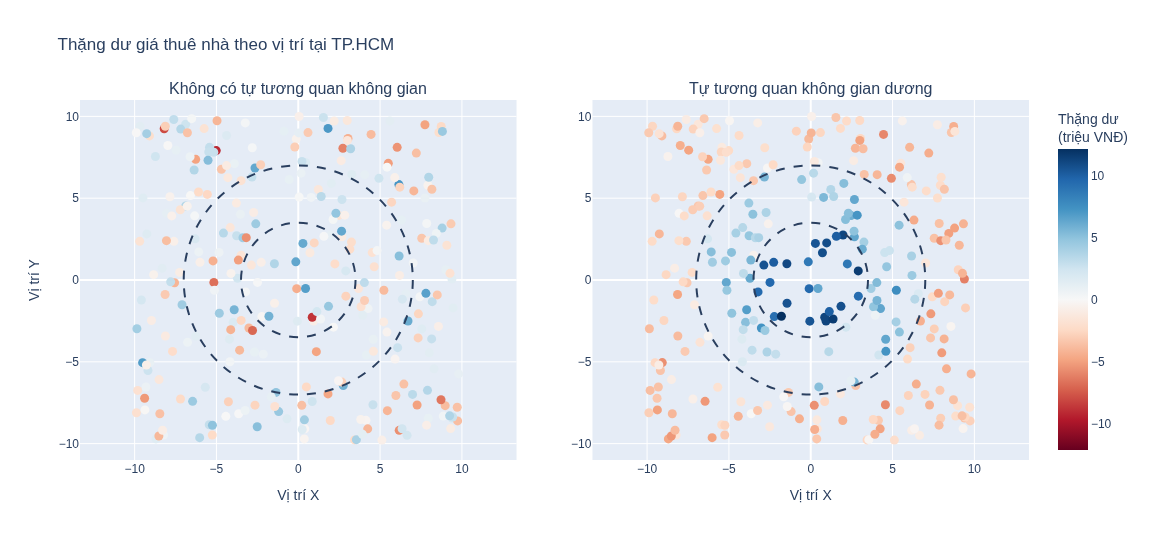
\includegraphics{media/rent_house.png}

Phương pháp đồ thị chỉ giúp nhận diện sơ bộ mẫu hình của thặng dư và có thể mang tính chủ quan. Vì vậy, kết luận chính thức cần dựa thêm trên các kiểm định thống kê phù hợp với loại dữ liệu.


\subsection{4.2. Kiểm định
Durbin-Watson}\label{kiux1ec3m-ux111ux1ecbnh-durbin-watson}

Kiểm định Durbin-Watson dùng để phát hiện tự tương quan bậc 1 trong
thặng dư của mô hình hồi quy. Nói cách khác, kiểm định này xem thặng dư
hiện tại có liên hệ tuyến tính với thặng dư ngay kỳ trước hay không.

Giả thuyết kiểm định thường được viết là:

\[
H_0:\rho=0 \quad \text{(không có tự tương quan bậc 1)}
\]
\[
H_1:\rho\neq 0,\quad \text{hoặc}\quad \rho>0,\quad \text{hoặc}\quad \rho<0
\]

tùy mục tiêu kiểm định

Trong đó:

\begin{itemize}
\item
  \(\rho\) là hệ số tự tương quan bậc 1 của sai số.
\item
  \(H_0\) biểu thị trường hợp không có tự tương quan bậc 1.
\item
  \(H_1\) biểu thị trường hợp có tự tương quan bậc 1; nếu kiểm định một phía
  thì có thể xét tự tương quan dương hoặc tự tương quan âm.
\end{itemize}

Sau khi ước lượng mô hình, ta lấy thặng dư \(e_t\) và tính thống kê
Durbin-Watson:

\[
d=\frac{\sum_{t=2}^{n}(e_t-e_{t-1})^2}{\sum_{t=1}^{n}e_t^2}
\]

Trong đó:

\begin{itemize}
\item
  d là thống kê Durbin-Watson.
\item
  \(e_t\) là thặng dư tại thời điểm t.
\item
  \(e_{t-1}\) là thặng dư tại thời điểm liền trước.
\item
  n là số quan trắc.
\item Tử số 
    $\sum_{t=2}^{n}(e_t - e_{t-1})^2$
    đo mức thay đổi giữa hai thặng dư liên tiếp.

\item Mẫu số 
    $\sum_{t=1}^{n} e_t^2$
    là tổng bình phương thặng dư, dùng để chuẩn hóa thống kê $d$.
\end{itemize}

Thống kê d có giá trị trong khoảng:

\[
0\le d\le 4
\]

Quan hệ gần đúng giữa thống kê d và hệ số tự tương quan mẫu bậc 1 là:

\[
d\approx 2(1-\hat{\rho})
\]

Trong đó \(\hat{\rho}\) là hệ số tự tương quan mẫu bậc 1 của thặng dư. Vì vậy:

\begin{itemize}
\item
  Nếu \(\hat{\rho}\approx 0\) thì \(d\approx 2\), tức chưa có dấu hiệu tự tương quan bậc 1 rõ ràng.
\item
  Nếu \(\hat{\rho}>0\) thì \(d<2\), tức nghi ngờ tự tương quan
  dương.
\item
  Nếu \(\hat{\rho}<0\) thì \(d>2\), tức nghi ngờ tự tương quan
  âm.
\item
  Nếu d gần 0 thì tự tương quan dương càng mạnh; nếu d gần 4 thì tự
  tương quan âm càng mạnh.
\end{itemize}

\subsection{Cách đọc kết quả bằng bảng
Durbin-Watson}\label{cuxe1ch-ux111ux1ecdc-kux1ebft-quux1ea3-bux1eb1ng-bux1ea3ng-durbin-watson}

Trong kiểm định Durbin-Watson, để kết luận chính thức theo bảng, ta so
sánh thống kê d với hai giá trị tới hạn \(d_L\) và \(d_U\).

Trong đó:

\begin{itemize}
\item
  \(d_L\) là cận dưới của bảng Durbin-Watson.
\item
  \(d_U\) là cận trên của bảng Durbin-Watson.
\item
  Hai giá trị này phụ thuộc vào số quan trắc n, số biến độc lập k trong
  mô hình và mức ý nghĩa \(\alpha\).
\end{itemize}

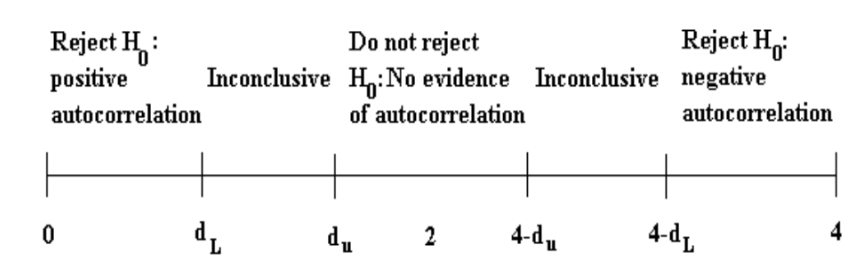
\includegraphics[width=5.7in,height=1.80588in]{media/image2.png}

Hình minh họa vùng quyết định của kiểm định Durbin-Watson.

Dựa vào sơ đồ vùng quyết định, ta đọc kết quả như sau:

\begin{itemize}
\item
  Nếu 0 < d < \(d_L\): bác bỏ \(H_0\), kết luận có tự tương
  quan dương.
\item
  Nếu \(d_L\) ≤ d ≤ \(d_U\): vùng không kết luận được.
\item
  Nếu \(d_U\) < d < 4 − \(d_U\): không bác bỏ \(H_0\), chưa có
  bằng chứng về tự tương quan.
\item
  Nếu 4 − \(d_U\) ≤ d ≤ 4 − \(d_L\): vùng không kết luận được.
\item
  Nếu 4 − \(d_L\) < d < 4: bác bỏ \(H_0\), kết luận có tự
  tương quan âm.
\end{itemize}

Nói cách khác, nếu d nằm gần 0 thì nghiêng về tự tương quan dương; nếu d
nằm gần 2 thì chưa có bằng chứng tự tương quan; nếu d nằm gần 4 thì
nghiêng về tự tương quan âm. Với kiểm định Durbin-Watson theo bảng, cần
tra \(d_L\) và \(d_U\) theo n, k và \(\alpha\).

Khi sử dụng R, hàm dwtest() trong gói lmtest cung cấp trực tiếp thống kê
d và p-value. Vì vậy, có thể kết luận dựa trên p-value thay vì tra bảng
thủ công.

Quy tắc đọc p-value là:

Nếu p-value < \(\alpha\) thì bác bỏ \(H_0\); nếu p-value ≥ \(\alpha\) thì chưa đủ cơ
sở bác bỏ \(H_0\).

\subsection{Hạn chế của kiểm định
Durbin-Watson}\label{hux1ea1n-chux1ebf-cux1ee7a-kiux1ec3m-ux111ux1ecbnh-durbin-watson}

Kiểm định Durbin-Watson chủ yếu phù hợp để phát hiện tự tương quan bậc
1. Nếu nghi ngờ tự tương quan bậc cao hơn, hoặc mô hình có biến phụ
thuộc trễ ở vế phải, kiểm định Durbin-Watson có thể không còn phù hợp.
Khi đó, kiểm định Breusch-Godfrey thường được sử dụng vì tổng quát hơn.

\subsection{4.3. Kiểm định
Breusch-Godfrey}\label{kiux1ec3m-ux111ux1ecbnh-breusch-godfrey}

Kiểm định Breusch-Godfrey tổng quát hơn Durbin-Watson vì có thể kiểm tra
tự tương quan đến bậc p và phù hợp hơn với các mô hình động. Giả sử sai
số có thể phụ thuộc vào p độ trễ:

\[
\varepsilon_t=\rho_1\varepsilon_{t-1}+\rho_2\varepsilon_{t-2}+\cdots+\rho_p\varepsilon_{t-p}+v_t
\]

Trong đó \(\rho_1\), \(\rho_2\), ..., \(\rho_p\) là các hệ số tự tương quan từ bậc 1 đến bậc p;
p là số độ trễ kiểm tra; \(v_t\) là nhiễu mới.

Giả thuyết kiểm định:

\[
H_0:\rho_1=\rho_2=\cdots=\rho_p=0
\]

\[
H_1:\text{ có ít nhất một }\rho_j\neq 0,\quad j=1,2,\ldots,p
\]

Vì không quan sát được \(\varepsilon_t\), ta dùng thặng dư \(e_t\) từ mô hình gốc và chạy
hồi quy phụ:

\[
e_t=\alpha_0+\alpha_1X_{1t}+\cdots+\alpha_kX_{kt}+\rho_1e_{t-1}+\cdots+\rho_pe_{t-p}+v_t
\]

Trong đó hồi quy phụ đưa lại các biến độc lập của mô hình gốc, rồi thêm
các thặng dư trễ. Mục tiêu là kiểm tra liệu các thặng dư trễ còn giải
thích được thặng dư hiện tại hay không.

Sau khi chạy hồi quy phụ, lấy \(R^2_{aux}\) là hệ số xác định của hồi quy phụ.
Thống kê LM là:

\[
LM=nR^2_{aux}
\]

Dưới \(H_0\) và với mẫu đủ lớn:

\[
LM\sim \chi^2(p)
\]

Trong đó \(\chi^2(p)\) là phân phối Chi-bình phương với \(p\) bậc tự do. Bác bỏ \(H_0\) nếu \(LM\) lớn hơn giá trị tới hạn \(\chi^2_{1-\alpha,p}\) hoặc p-value nhỏ hơn \(\alpha\). Khi
bác bỏ \(H_0\), ta kết luận có bằng chứng thống kê về tự tương quan đến bậc
p.

Việc chọn p không nên tùy ý. p nên dựa vào tần suất dữ liệu, bản chất
bài toán hoặc đồ thị ACF/PACF của thặng dư. Ví dụ với dữ liệu tháng, p =
12 có thể dùng để kiểm tra phụ thuộc theo cùng tháng của năm trước, tức
cấu trúc mùa vụ hằng năm.

\subsection{4.4. Kiểm định tự tương quan trên R}

Để minh họa việc phát hiện tự tương quan, mô hình hồi quy doanh thu bán hàng được ước lượng như sau:

\[
\mathrm{sales\_revenue}_t
=
\beta_0
+
\beta_1\mathrm{advertising\_cost}_t
+
\beta_2\mathrm{discount\_rate}_t
+
\varepsilon_t
\]

Trong đó, $\mathrm{sales\_revenue}_t$ là doanh thu bán hàng tại tháng $t$,
$\mathrm{advertising\_cost}_t$ là chi phí quảng cáo và
$\mathrm{discount\_rate}_t$ là tỷ lệ giảm giá.

Mô hình được ước lượng bằng hàm \texttt{lm()} trong R:

\begin{lstlisting}[language=R]
sales_model <- lm(
  sales_revenue ~ advertising_cost + discount_rate,
  data = sales_data
)

summary(sales_model)

res <- residuals(sales_model)
\end{lstlisting}

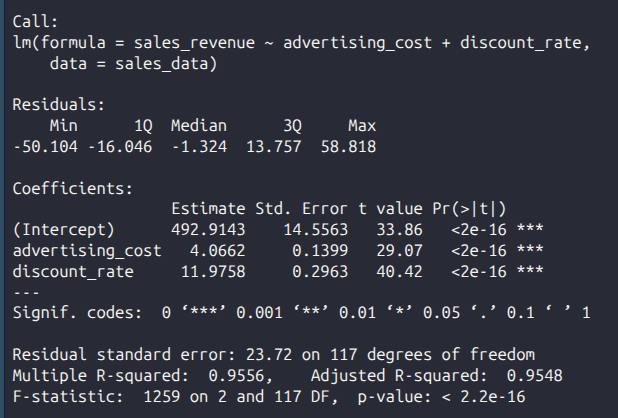
\includegraphics{media/summary.png}

Kết quả ước lượng thu được phương trình:

\[
\widehat{\mathrm{sales\_revenue}}_t
=
492.9143
+
4.0662\,\mathrm{advertising\_cost}_t
+
11.9758\,\mathrm{discount\_rate}_t
\]

Khi giữ các yếu tố khác không đổi, kết quả có thể được diễn giải như sau:

\begin{itemize}
    \item Khi chi phí quảng cáo tăng một đơn vị, doanh thu ước lượng tăng trung bình khoảng $4.0662$ đơn vị.
    
    \item Khi tỷ lệ giảm giá tăng một điểm phần trăm, doanh thu ước lượng tăng trung bình khoảng $11.9758$ đơn vị.
\end{itemize}

Đối với từng hệ số, các p-value đều nhỏ hơn $2\times10^{-16}$. Vì vậy, ở mức ý nghĩa $5\%$, các hệ số của chi phí quảng cáo và tỷ lệ giảm giá đều có ý nghĩa thống kê.

Hệ số xác định của mô hình là:

\[
R^2
=
0.9556
\]

Điều này có nghĩa là khoảng $95.56\%$ biến động của doanh thu trong dữ liệu mẫu được giải thích bởi chi phí quảng cáo và tỷ lệ giảm giá.

Kiểm định F về ý nghĩa thống kê chung của mô hình cho kết quả:

\[
F
=
1259
\]

với p-value nhỏ hơn $2.2\times10^{-16}$. Do đó, ta bác bỏ giả thuyết:

\[
H_0:
\beta_1
=
\beta_2
=
0
\]

và kết luận rằng xét chung, chi phí quảng cáo và tỷ lệ giảm giá có ý nghĩa thống kê trong việc giải thích doanh thu bán hàng.

Sai số chuẩn thặng dư của mô hình là:

\[
23.72
\]

cho biết mức chênh lệch điển hình giữa doanh thu thực tế và doanh thu được mô hình ước lượng vào khoảng $23.72$ đơn vị.

Nhìn chung, kết quả ban đầu cho thấy mô hình phù hợp tốt với dữ liệu mô phỏng: các hệ số ước lượng gần với giá trị được đặt trước, các biến độc lập đều có ý nghĩa thống kê, $R^2$ cao và kiểm định F cho thấy mô hình có ý nghĩa chung.

\subsubsection{Kiểm định Durbin--Watson}

Kiểm định Durbin--Watson được thực hiện bằng hàm \texttt{dwtest()} trong
gói \texttt{lmtest}:

\begin{lstlisting}[language=R]
library(lmtest)

dwtest(sales_model)
\end{lstlisting}

Giả thuyết kiểm định là:

\[
H_0:
\rho = 0
\quad
\text{(không có tự tương quan dương bậc 1)}
\]
\[
H_1:
\rho > 0
\quad
\text{(có tự tương quan dương bậc 1)}
\]

Kết quả kiểm định thu được:

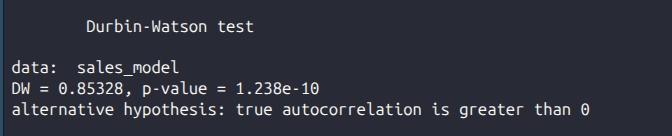
\includegraphics{media/d.png}

Do p-value nhỏ hơn mức ý nghĩa $5\%$, ta bác bỏ giả thuyết $H_0$.
Ngoài ra, giá trị Durbin--Watson nhỏ hơn $2$ và tương đối gần $0$, cho
thấy thặng dư có dấu hiệu tự tương quan dương.

Như vậy, kiểm định Durbin--Watson cung cấp bằng chứng thống kê rằng thặng
dư của mô hình có tự tương quan dương bậc 1.

\subsubsection{Kiểm định Breusch--Godfrey}

Để kiểm tra tự tương quan tổng quát hơn, kiểm định Breusch--Godfrey được
thực hiện bằng hàm \texttt{bgtest()}.

Kiểm định tự tương quan đến bậc 1 được thực hiện như sau:

\begin{lstlisting}[language=R]
bgtest(sales_model, order = 1)
\end{lstlisting}

Giả thuyết kiểm định là:

\[
H_0:
\rho_1 = 0
\]
\[
H_1:
\rho_1 \neq 0
\]

Kết quả thu được:

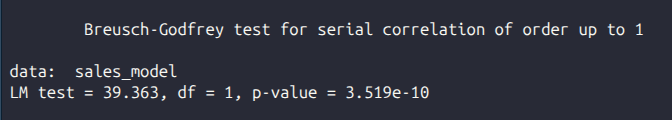
\includegraphics{media/bg_1.png}

Do p-value nhỏ hơn $0.05$, ta bác bỏ $H_0$ và kết luận có bằng chứng về
tự tương quan đến bậc 1.

Tiếp theo, kiểm định tự tương quan đến bậc 2 được thực hiện bằng:

\begin{lstlisting}[language=R]
bgtest(sales_model, order = 2)
\end{lstlisting}

Giả thuyết kiểm định là:

\[
H_0:
\rho_1
=
\rho_2
=
0
\]
\[
H_1:
\text{có ít nhất một hệ số }
\rho_j
\neq
0,
\qquad
j=1,2
\]

Kết quả thu được:

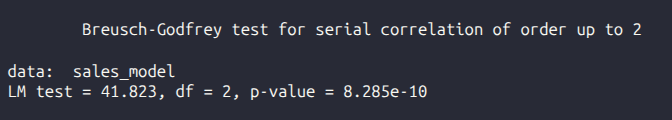
\includegraphics{media/bg_2.png}

Do p-value nhỏ hơn $0.05$, ta bác bỏ giả thuyết không có tự tương quan
đến bậc 2.

Kết quả kiểm định bậc 2 cho thấy trong các hệ số tự tương quan
$\rho_1$ và $\rho_2$, có ít nhất một hệ số khác $0$. Kết quả này không
có nghĩa là riêng hệ số tự tương quan bậc 2 chắc chắn có ý nghĩa thống kê.

\subsubsection{Kết luận}

Cả kiểm định Durbin--Watson và Breusch--Godfrey đều bác bỏ giả thuyết
không có tự tương quan. Vì vậy, có bằng chứng thống kê mạnh cho thấy
thặng dư của mô hình doanh thu bán hàng tồn tại tự tương quan dương.

Mặc dù mô hình có $R^2$ cao và các biến độc lập đều có ý nghĩa thống kê,
sự tồn tại của tự tương quan làm cho các sai số chuẩn, p-value và kết quả
suy luận OLS thông thường có thể không còn đáng tin cậy.

\section{Tài liệu tham khảo}\label{tuxe0i-liux1ec7u-tham-khux1ea3o}

Gujarati, D. N., \& Porter, D. C. (2009). Basic Econometrics (5th ed.).
McGraw-Hill. Chapter 12: Autocorrelation: What Happens If the Error
Terms Are Correlated?

\end{document}